%\input{Preambulum}

\begin{figure}[t!]
\centering

\begin{subfigure}{\textwidth}
\caption{With pair constraints}
\label{Fig8a}

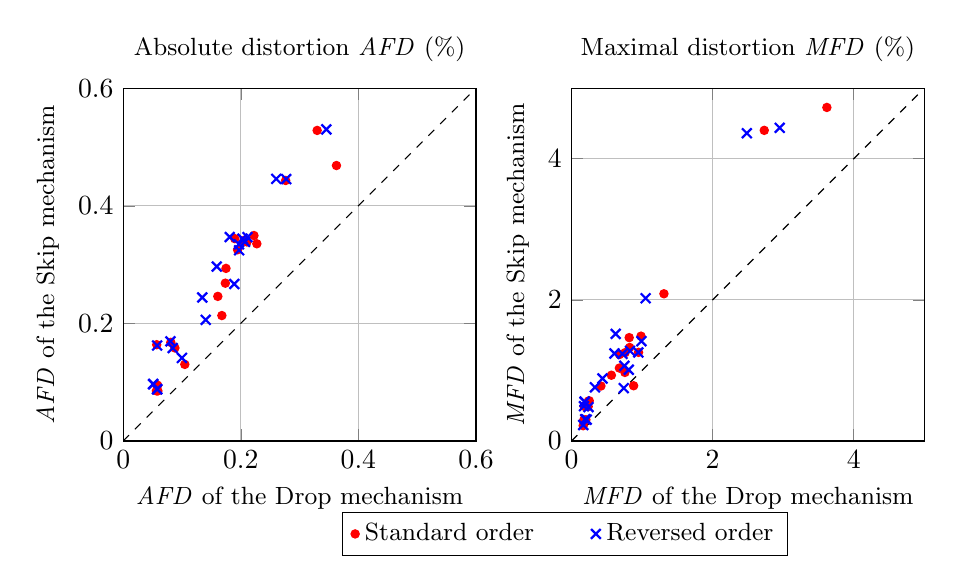
\begin{tikzpicture}
\begin{axis}[
name = axis1,
title = {Absolute distortion $\mathit{AFD}$ (\%)},
title style = {font=\small},
xlabel = $\mathit{AFD}$ of the Drop mechanism,
x label style = {font=\small},
ylabel = $\mathit{AFD}$ of the Skip mechanism,
y label style = {font=\small},
width = 0.5\textwidth,
height = 0.5\textwidth,
nodes near coords,
xmajorgrids = true,
ymajorgrids = true,
xmin = 0,
xmax = 0.6,
ymin = 0,
ymax = 0.6,
]
\addplot [scatter,red,only marks,mark size=1.5pt,point meta=explicit symbolic] coordinates {
(0.104803637938864,0.130297902089807)
(0.276309721518334,0.44301580571218)
(0.0879416390484003,0.158262119770303)
(0.0809882958117887,0.16775080561571)
(0.189760612931133,0.344121772673117)
(0.222393175891974,0.349458265991503)
(0.0565348702482663,0.0852635952960898)
(0.17483359530208,0.293552928635414)
(0.0585406557299952,0.0947755685604725)
(0.173740611861615,0.268416024909391)
(0.0570315137975406,0.163795486202459)
(0.167812786572911,0.213345442562499)
(0.0571245802582969,0.0946287846639068)
(0.194517975192498,0.325220540477796)
(0.362699791507353,0.468469065269525)
(0.22730844506906,0.335398178483798)
(0.210541863253026,0.338492808958483)
(0.205475622235813,0.341182227572666)
(0.160939514361695,0.24594437400595)
(0.329871531905745,0.528165483273134)
(0.0589570915351405,0.0851857952388442)
};
\addplot [scatter,blue,only marks,mark=x,mark size=2.5pt,thick,point meta=explicit symbolic] coordinates {
(0.0998811473728264,0.14131741152377)
(0.277183362609177,0.445430957280265)
(0.0841283822805577,0.158074761279737)
(0.0803465311059063,0.169446962478455)
(0.181238400478088,0.346832132673117)
(0.21144495820965,0.346781787730633)
(0.0574450292583537,0.088232991522505)
(0.159120497262865,0.296689399223649)
(0.0509923439214011,0.096728990455681)
(0.188986339769358,0.267003144909391)
(0.0577002637975405,0.162378819535793)
(0.140329873393467,0.206054381338009)
(0.0510484596413713,0.0969411328428128)
(0.197202619859371,0.324335786261676)
(0.260335718330749,0.445728575473606)
(0.196880700388209,0.334495421142969)
(0.207267692679414,0.338672297330576)
(0.203052655100267,0.344081631827985)
(0.134491888282274,0.244106340224272)
(0.345524098899209,0.529904524939801)
(0.0580508693129183,0.0879172026462514)
};
% Zero line
\draw [black,dashed] (rel axis cs:0,0) -- (rel axis cs:1,1);
\end{axis}

\begin{axis}[
at = {(axis1.south east)},
xshift = 0.1\textwidth,
title = {Maximal distortion $\mathit{MFD}$ (\%)},
title style = {font=\small},
xlabel = $\mathit{MFD}$ of the Drop mechanism,
x label style = {font=\small},
ylabel = $\mathit{MFD}$ of the Skip mechanism,
y label style = {font=\small},
width = 0.5\textwidth,
height = 0.5\textwidth,
nodes near coords,
xmajorgrids = true,
ymajorgrids = true,
xmin = 0,
xmax = 5,
ymin = 0,
ymax = 5,
legend style = {font=\small,at={(-0.65,-0.2)},anchor=north west,legend columns=3},
legend entries = {Standard order$\qquad$,Reversed order}
]
\addplot [scatter,red,only marks,mark size=1.5pt,point meta=explicit symbolic] coordinates {
(0.16576483482775,0.21645683482775)
(0.950310657084946,1.2566682937166)
(0.417101695652172,0.779423695652173)
(0.236011323065366,0.488418323065365)
(0.817866827546956,1.46537791083286)
(0.985194267737621,1.4861098433735)
(0.175163831977129,0.298908831977129)
(0.565436893401014,0.932306893401014)
(0.251600376626215,0.570317376626217)
(0.757380291231924,0.971869031850631)
(0.176731291392623,0.493903708607379)
(0.880524062001772,0.783162062001772)
(0.239471376626216,0.564707376626217)
(0.678622224507283,1.03384822450728)
(3.61906849551675,4.72712549551675)
(0.82454974066053,1.32544474066053)
(0.758948317682318,1.25173931768232)
(0.681065974281392,1.22652858850227)
(1.31018118510772,2.08649918510772)
(2.73182211455109,4.40232811455108)
(0.20401683482775,0.301104834827751)
};
\addplot [scatter,blue,only marks,mark=x,mark size=2.5pt,thick,point meta=explicit symbolic] coordinates {
(0.166456033034451,0.22643283482775)
(0.947172657084946,1.25466728689884)
(0.332109695652175,0.760869695652175)
(0.241466213373404,0.480888323065365)
(0.626087910832862,1.51842691083286)
(0.991432267737619,1.41423126773762)
(0.193966831977127,0.309116831977127)
(0.439313893401017,0.886105893401012)
(0.186033376626216,0.559111376626215)
(0.811668031850632,1.01026103185063)
(0.177210291392621,0.493557708607378)
(0.740216062001772,0.749893062001772)
(0.187383961080137,0.553348376626217)
(0.749596570694089,1.06552857069409)
(2.48499449551675,4.36220749551675)
(0.60985178180834,1.24009974066053)
(0.721625317682317,1.23551331768232)
(0.828914588502266,1.27715858850227)
(1.05080918510772,2.02340218510771)
(2.95084211455108,4.43835211455108)
(0.215691033034451,0.302748834827749)
};
% Zero line
\draw [black,dashed] (rel axis cs:0,0) -- (rel axis cs:1,1);
\end{axis}
\end{tikzpicture}
\end{subfigure}

\vspace{0.25cm}
\begin{subfigure}{\textwidth}
\caption{Without pair constraints}
\label{Fig8b}

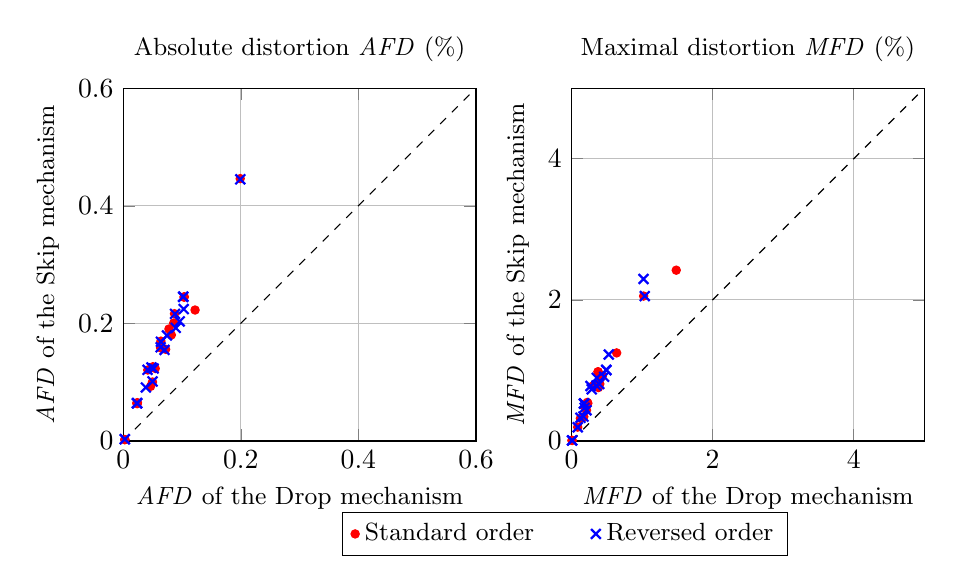
\begin{tikzpicture}
\begin{axis}[
name = axis1,
title = {Absolute distortion $\mathit{AFD}$ (\%)},
title style = {font=\small},
xlabel = $\mathit{AFD}$ of the Drop mechanism,
x label style = {font=\small},
ylabel = $\mathit{AFD}$ of the Skip mechanism,
y label style = {font=\small},
width = 0.5\textwidth,
height = 0.5\textwidth,
nodes near coords,
xmajorgrids = true,
ymajorgrids = true,
xmin = 0,
xmax = 0.6,
ymin = 0,
ymax = 0.6,
]
\addplot [scatter,red,only marks,mark size=1.5pt,point meta=explicit symbolic] coordinates {
(0.0027159718969553,0.00236561124121789)
(0.103840630541872,0.245321320197044)
(0.0505506666666667,0.126349133333334)
(0.0418565164506482,0.120754488534397)
(0.1035639408867,0.244561802955665)
(0.0721563673933977,0.155964870414149)
(0.0231160230394329,0.0644587771377934)
(0.0819136271186443,0.180416813559322)
(0.0242181869738591,0.0651744492689409)
(0.0641531414180552,0.169859175900814)
(0.199030521264995,0.446227092693566)
(0.0872722807017539,0.216451349527665)
(0.0239509738591049,0.0635049410722198)
(0.063600871737786,0.158487444650587)
(0.122241219744276,0.222776861135891)
(0.0465788381504286,0.0929222941446337)
(0.0498328755376162,0.100351682921988)
(0.0859359494607086,0.200570981201849)
(0.0545282083367541,0.123337861619728)
(0.0778373703703707,0.190472547619048)
(0.00295612903225803,0.00246284792626718)
};
\addplot [scatter,blue,only marks,mark=x,mark size=2.5pt,thick,point meta=explicit symbolic] coordinates {
(0.00261861358313812,0.00320835597189687)
(0.102261596059113,0.245558492610837)
(0.0481568666666669,0.125018733333334)
(0.0414737427716851,0.121105539381854)
(0.102004837438424,0.245099251231527)
(0.0703760605901405,0.154937777602661)
(0.0235591705804164,0.0642886787771377)
(0.0744606779661017,0.179448406779661)
(0.0233000886132033,0.0642198918918917)
(0.0642319345215034,0.168775313831848)
(0.19914530697928,0.445036021264995)
(0.0880725677013042,0.216215209176788)
(0.0238123509082853,0.0644630394328755)
(0.0636542899196041,0.159447808286951)
(0.102957779958371,0.224423738328873)
(0.0385748109622119,0.0911320032355428)
(0.0499460520082047,0.101327834623613)
(0.0961051500770417,0.203415267180277)
(0.0517399022360892,0.123374072146043)
(0.0894688240740743,0.192321714285714)
(0.00281358218125953,0.00300070967741932)
};
% Zero line
\draw [black,dashed] (rel axis cs:0,0) -- (rel axis cs:1,1);
\end{axis}

\begin{axis}[
at = {(axis1.south east)},
xshift = 0.1\textwidth,
title = {Maximal distortion $\mathit{MFD}$ (\%)},
title style = {font=\small},
xlabel = $\mathit{MFD}$ of the Drop mechanism,
x label style = {font=\small},
ylabel = $\mathit{MFD}$ of the Skip mechanism,
y label style = {font=\small},
width = 0.5\textwidth,
height = 0.5\textwidth,
nodes near coords,
xmajorgrids = true,
ymajorgrids = true,
xmin = 0,
xmax = 5,
ymin = 0,
ymax = 5,
legend style = {font=\small,at={(-0.65,-0.2)},anchor=north west,legend columns=3},
legend entries = {Standard order$\qquad$,Reversed order}
]
\addplot [scatter,red,only marks,mark size=1.5pt,point meta=explicit symbolic] coordinates {
(0.00747357142857202,0.00789942857142845)
(0.375094428571426,0.981217428571426)
(0.194242,0.478719999999999)
(0.126345117647059,0.321747117647059)
(0.378572428571428,0.979924428571427)
(0.412635501182032,0.909821501182032)
(0.22726191891892,0.539132918918919)
(0.381924222222221,0.757366222222222)
(0.223651918918921,0.54694191891892)
(0.173916966292134,0.343732966292135)
(0.354852412213738,0.788794412213739)
(0.304277333333333,0.780359333333333)
(0.230854918918921,0.535309918918919)
(0.212871734693876,0.437639734693876)
(1.48455757627119,2.42082757627119)
(0.401224270916337,0.809733270916335)
(0.0877381361079871,0.196886136107985)
(0.437903745762711,0.923035084745763)
(0.640268238689545,1.24876423868955)
(1.02232277777778,2.05421077777778)
(0.00821009523809535,0.00921671428571469)
};
\addplot [scatter,blue,only marks,mark=x,mark size=2.5pt,thick,point meta=explicit symbolic] coordinates {
(0.00839671428571609,0.00829657142857182)
(0.495235428571428,1.00458342857143)
(0.185794,0.471757)
(0.127171117647057,0.328761117647058)
(0.491708428571427,1.00932242857143)
(0.358447460992908,0.894296501182032)
(0.177274918918921,0.52876991891892)
(0.28669922222222,0.732984222222222)
(0.178743918918919,0.52825791891892)
(0.168894966292135,0.346142966292134)
(0.353426412213739,0.78663141221374)
(0.394191333333335,0.807164333333335)
(0.17940691891892,0.53340991891892)
(0.213547734693875,0.435606734693877)
(1.02097857627119,2.29616557627119)
(0.269174270916336,0.779243270916335)
(0.0886461361079866,0.194942136107987)
(0.461847745762711,0.910904084745764)
(0.528509238689545,1.22566923868955)
(1.03879577777778,2.05351277777778)
(0.00960590476190432,0.00822328571428443)
};
% Zero line
\draw [black,dashed] (rel axis cs:0,0) -- (rel axis cs:1,1);
\end{axis}
\end{tikzpicture}
\end{subfigure}

\caption{Fairness distortions of the draw mechanisms, graphs corresponding to the UEFA Champions League Round of 16 from 2003/04 to 2023/24}
\label{Fig8}
\end{figure}

%\end{document}